\chapter{Robot Verbal Immediacy and Child Learning} \label{chap:verbal}

\begin{framed}
	\textbf{Key points:}
	
	\begin{itemize}
	\item High \gls{nonverbalimm} behaviours applied to social robot tutors have been found to lead to significant child \gls{learning} in the previous chapter. This chapter now considers the other part of the immediacy construct: \gls{verbalimm}.
	\item A novel French language learning scenario is devised. Building on methodological approaches from previous chapters, a recall test is completed by the children the following week in addition to the pre-test and post-test as part of the interaction. A greater number of subjects are also considered in this experiment.
	\item It is found that children learn a significant amount in both high and low \gls{verbalimm} conditions. However, despite being able to perceive differences in \gls{verbalimm}, child \gls{learning} is equivalent between conditions.
	\item Children retain their \gls{learning} the following week and acquire vocabulary during the interaction, highlighting the promise of applying social robots in the context of language learning.
	\end{itemize}
\end{framed}

Part of the work presented in this chapter has been published in \cite{kennedy2016social}. The final publication is available from the IEEE via: \newline http://dx.doi.org/10.1109/HRI.2016.7451757

\newpage
Previous chapters have explored the impact of nonverbal social behaviour and \gls{nonverbalimm} on \gls{learning}. Of course, this only covers part of the immediacy construct, with a range of \gls{verbalimm} behaviours remaining unexplored in \acrshort{hri}. This chapter seeks to evaluate the impact of verbal social behaviour, as motivated by \gls{verbalimm}, on child \gls{learning}. An experiment is devised to test this, which builds upon the methodological approaches taken in previous chapters. The \gls{learning} of the children is measured in the short-term (immediately after the interaction), and also the following week to check that the learned information is retained.

This chapter also introduces a novel language learning task. Child language learning provides an ideal domain for social \acrshort{hri} to contribute to. In the case of language, children learn better than adults, despite the increased cognitive capacity of adults. Language learning has a `critical period' in neurobiology \citep{kuhl2010brain}, which means that there is a window in which it is best learned. As such, evaluating with children aged 8 and 9 years old as in previous chapters is ideal. At this age, the children are still within the critical period, but have sufficient skill to read novel words without assistance. Language learning is an inherently social process \citep{kuhl2007cracking}, which places it in a strong position to evaluate social behaviour. It is hoped that by making the task rely more heavily on social behaviour, the robot can have a greater influence on the outcome of the \gls{learning}. 

The background for this thesis provided in Chapter \ref{chap:background} introduced a variety of work conducted in the field of \acrshort{hri} with a focus on the impact of robot social behaviour, and where possible, how this related to \gls{learning} outcomes. As the work in this chapter moves into the domain of language learning, literature from \acrshort{hri} focusing on this will now be discussed to inform the experimental design here. Some of the literature has previously been referenced in Chapter \ref{chap:background}, but will be considered from a different perspective here, with a focus on the types of tasks and \gls{learning} taking place.

%%%%%%%%%%%%%%%%%%%%%%%%%%%%%%%%%%%%%%%%%%%%%%%%%%%%%%%%%%%%%%%%%%%%%%%%%%%%%%
\section{Language Learning and Social Robots}
Using social robots to teach a foreign language has been explored by different researchers with various aims. This section will discuss studies with children for the purpose of informing the design of the experiment in this chapter, and to provide context for the findings here. A summary of the studies considered in this section can be seen in Table \ref{tab:ch9-litrev}.

\afterpage{%
	\begin{landscape}
		\begin{table}[t]
		\centering
		\renewcommand{\arraystretch}{1.2} 
		\begin{tabulary}{1.6\textwidth}{@{}Lp{2.2cm}L>{\raggedright}p{0.92cm}LLL@{}}
		\toprule
		Reference & Language & Aspect & Child Age & n & Research Topic & Details/outcomes \\ \midrule
		\cite{alemi2014employing} & English (L2) & Vocabulary & 12 & 60 & Robot presence & 5 week, multi session study. Children learn significantly more when robot is present \\
		\cite{gordon2015curiosity} & English (L1) & Vocabulary & 3-8 & 48 & Social behaviour (curiosity), Embodiment (robot/tablet) & Learning was significant (above chance), but averaged 1 word per interaction \\
		\cite{herberg2015robot} & French, Latin & Verb conjugations & 10-12 & 23 & Social behaviour (watchfulness) & Being watched by the robot leads to less learning, but there is a potential confound in terms of general motion \\
		\cite{kanda2004interactive} & English (L2) & Vocabulary & 6-7, 11-12 & 119, 109 & Robot presence & 2 week study. No overall learning effect, but effect for children who interact more with the robot in the second week. \\
		\cite{westlund2015comparison} & English (L1) & Vocabulary & 4-6 & 19 & Embodiment (robot/tablet/human) & Learning equal, but only 6 words are used \\
		\cite{saerbeck2010expressive} & Toki Pona & Pronunciation, Vocabulary, Grammar & 10-11 & 16 & Social behaviour (socially supportive) & Significant learning is observed for the robot with socially supportive behaviours \\
		\cite{tanaka2012children} & English (L2) & Vocabulary & 3-6 & 17 & Robot presence & Significantly greater learning when interacting with a robot compared to when not \\ \bottomrule
		\end{tabulary}
		\caption{A summary of studies conducted in \acrshort{hri} to investigate different aspects of robots on child language learning. \textit{L1} indicates where English was being taught to native speakers, whereas \textit{L2} refers to cases where English was being taught as a foreign language.}
		\label{tab:ch9-litrev}
		\end{table}
	\end{landscape}
}

\cite{alemi2014employing} employed a social robot as an assistant to a teacher over a 5 week period to teach English vocabulary to Iranian students. It was found that the class with the robot assistant learnt significantly more than those with just the human teacher. In addition, this vocabulary was retained, as measured through a retention test. This builds on earlier findings by \cite{kanda2004interactive} where a 2 week study with a robot situated in the classroom revealed a connection between interacting with a robot and vocabulary acquisition. Further results by \cite{tanaka2012children} also confirm that the presence of a robot leads to significant \gls{learning} of vocabulary. All three of these studies used children learning English as a second language and took place `in the wild', with child ages ranging from 3 to 12.

Other researchers have explored the impact of embodiment and social behaviour for children learning English as a first language in a laboratory setting. Neither \cite{gordon2015curiosity} or \cite{westlund2015comparison} found significant differences due to embodiment in their studies of vocabulary acquisition by children. However, this may be due in part to methodological limitations. \cite{gordon2015curiosity} only find an average of 1 word learnt per interaction, leaving very little room for observing differences; similarly \cite{westlund2015comparison} only compares the learning of 6 words. These studies were conducted with children aged between 3 and 8. The relatively small gains are therefore quite surprising, due to the speed at which children of this age can theoretically acquire language \citep{kuhl2010brain}. Due to the novelty of methodologies and comparison with both tablets and humans, it is suggested that the small learning gains are likely not due to the use of a robot.

Social behaviour has previously been studied in the context of children learning languages that were novel to them. \cite{saerbeck2010expressive} explored the impact of `socially supportive' behaviours on child learning of the Toki Pona language, using an iCat as the tutor. These behaviours included verbal and non-verbal manipulations which aimed to influence feedback provision, attention guiding, empathy and communicativeness. It was found that the tutor with these socially supportive behaviours led to significantly greater child learning when compared to a neutral tutor. This study used a variety of measures including vocabulary acquisition, as other studies have, but also included pronunciation and grammar tests. Another study which did not consider only vocabulary acquisition can be seen in \cite{herberg2015robot}. French and Latin verb conjugations were taught by an Aldebaran NAO to children aged 10-12. In one condition, the robot would look towards the student whilst they completed worksheets, but in the other, the robot would look away. While gaze towards the child was predicted to lead to greater social facilitation effects (and therefore higher performance), this was not found.

As discussed in Chapter \ref{chap:background}, certain aspects of \gls{verbalimm} have previously been explored in \acrshort{hri}. However, these research efforts did not frame the work in terms of immediacy, or focus on learning. Nevertheless, they provide promising indications of positive outcomes when applying high \gls{verbalimm} social behaviour on robots interacting with children. It has been found that `off-activity talk' - dialogue with a robot which does not concern the task being completed - encourages compliance in children in a therapeutic setting \citep{kruijff2014oat}. Personalisation in therapeutic contexts has also been considered. Children were asked a number of questions about their preferences and the robot then mentioned these in an interaction, the children who interacted with a personalised robot enjoyed the interaction more, but subject numbers were too low for statistical comparisons \citep{henkemans2013using}.

In summary, many promising results have been found when robots have been used to tutor children aspects of language. The presence of a robot produces clear advantages when tutoring \citep{alemi2014employing,kanda2004interactive,tanaka2012children}. However, the impact of social behaviour is less clear, with some positive results \citep{saerbeck2010expressive}, but other negative ones \citep{herberg2015robot}. Verbal immediacy will be used in this chapter to further explore the impact of robot social behaviour on child language learning. Despite an increasing interest, there are still relatively few studies that have considered robot language tutoring, leaving space to explore novel aspects of language learning, which will be done here.

%%%%%%%%%%%%%%%%%%%%%%%%%%%%%%%%%%%%%%%%%%%%%%%
\section{Hypothesis}\label{sec:verbal-hyp}
Following on from previous research with humans \citep{gorham1988relationship} and robots \citep{henkemans2013using,kruijff2014oat} this chapter aims to test whether robot \gls{verbalimm} has a positive impact on children's second language learning as predicted by the literature. In order to make such an assessment, it first needs to be clear that children perceive the behaviour of the robot as intended, so a manipulation check will be conducted. Verbal immediacy provides a basis for measuring the children's perceptions and also for motivating differences between robot conditions. To ensure that any observed \gls{learning} effects are retained and not just the product of short-term memory recall, the aim is also to verify children's retention of the material outside of the short-term interaction context (as in \citealt{tanaka2012children}). As such, the hypothesis below will be tested in the short-term, and after a delayed period:

\begin{enumerate}
\setlength\itemsep{0.05em}
	\item[\textbf{H1}:] A robot exhibiting more \gls{verbalimm} behaviour will lead to greater child learning gains than a robot without this behaviour.
\end{enumerate}

\begin{figure}[t!]
    \centering
    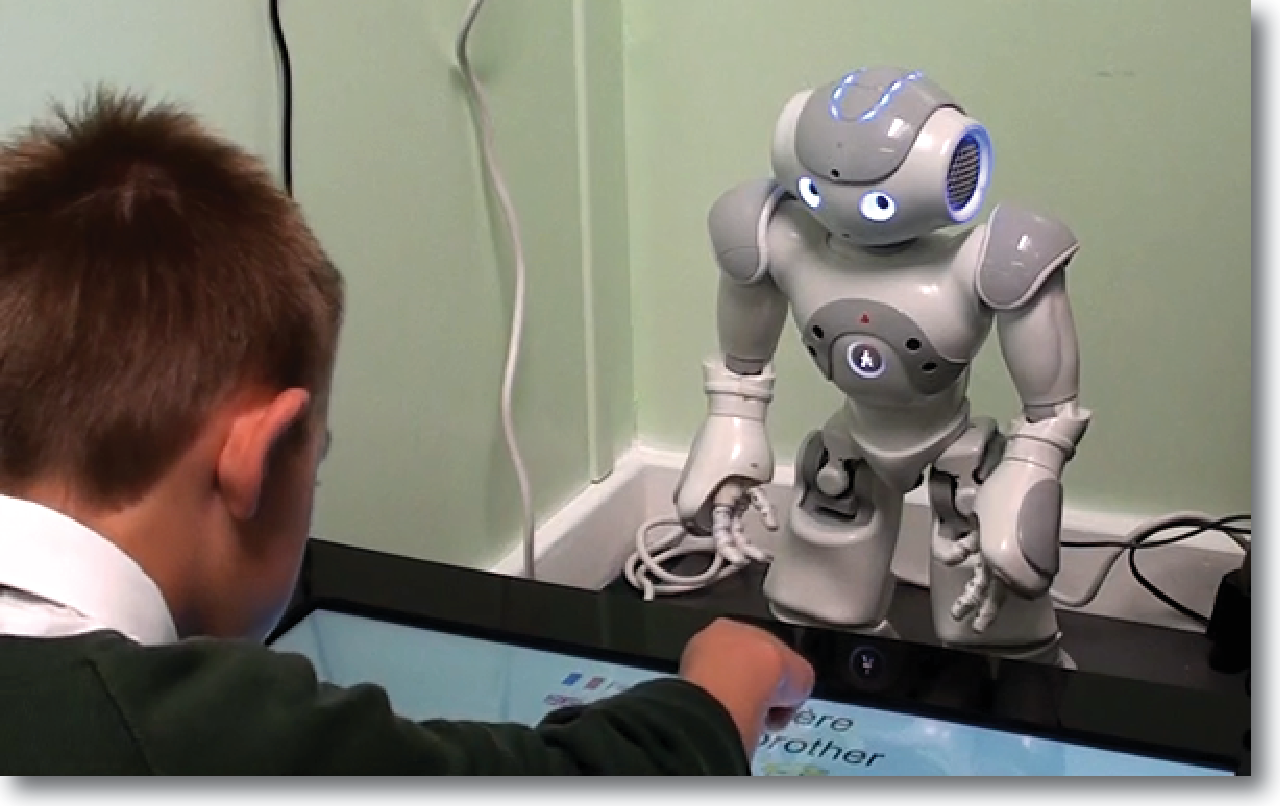
\includegraphics[width=0.75\textwidth]{images/ch9_Snapshot.pdf}
    \caption{A child answering a question on screen during the interaction.}
    \label{fig:snapshot}
\end{figure}

%%%%%%%%%%%%%%%%%%%%%%%%%%%%%%%%%%%%%%%%%%%%%%%
\section{Experimental Setup} \label{sec:verbal-setup}
The study used 2 robot conditions (high vs. low verbal immediacy) in a between-subjects design, with an additional control condition (no intervention) to verify that a practice effect was not introduced from exposure to the learning test. French is commonly taught in English schools, so would have clear relevance for the children. However, it does not receive very much lesson time (the majority of schools offer 30-45 minutes per week at the age used in this study; \citealp{board2015language}), so there is plenty of scope to teach new concepts. As such, French was selected as the second language to teach in this study. The learning material was developed in collaboration with an academic researcher in language development, a native French speaker, and a teacher.

The structure of the lesson content was designed based on previous work in which children learnt mathematical concepts, such as \cite{kennedy2015robot}, and a pilot study involving a human tutor and children. The aim was for the children to learn that nouns in French have a gender, that this changes which article is used (`le' or `la'), and that for some words there are patterns which can be used to help work out which article to use. This is a novel learning topic for \acrshort{hri}.

An Aldebaran NAO robot acted as a tutor, delivering all lessons through speech and moving words on a touchscreen (Figure \ref{fig:snapshot}). As such, the children were exposed to both the words' pronunciation and orthography. The robot demonstrated how questions could be answered by dragging and dropping the correct answer in the blank space (see Figure \ref{fig:screenshot}). The robot first explained the concept of words having a gender by using an English example (using `waiter' for a man, and `waitress' for a woman). Following this, it explained how the French word for `the' could be `le' or `la' depending on the gender of the noun it precedes. The robot then explained rules for working out whether to use `le' or `la'. After explaining each rule, the child's understanding was checked (Figure \ref{fig:taskstruct}). 

\begin{figure}[t!]
    \centering
    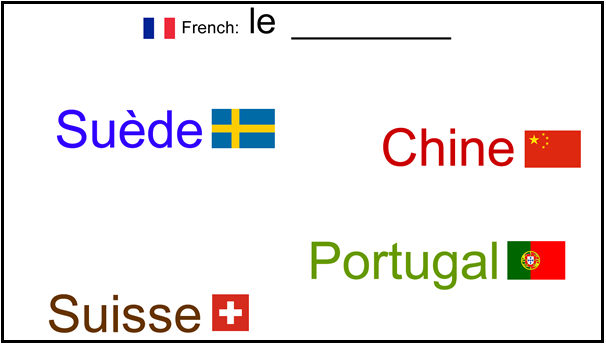
\includegraphics[width=0.75\textwidth]{images/ch9_Screenshot.png}
    \caption{Screenshot from the touchscreen showing a question. Children can touch a word, drag it to the blank space and release to answer. Here the correct answer being `Portugal'.}
    \label{fig:screenshot}
\end{figure}

During the lessons the robot would explain a rule and then use the screen to show an example. The rules used were taken from online French language learning guides\footnote{\label{note1}\url{http://goo.gl/JPjmPO}}$^{,}$\footnote{\label{note2}\url{https://goo.gl/WY37z5}} and were verified by a French native speaker. The rules were as follows: 1) `le' is used for male people, and `la' is used for female people, 2) `la' is used for countries ending in `e', 3) `la' is used for fruit or vegetables ending in `e'. Whilst these are recognised techniques for people learning a second language, it should be made clear that it is unlikely that a native speaker would learn in this way, and that there are a limited number of exceptions to rules 2 and 3 (but these were avoided in the lesson content here). As described in Chapter \ref{chap:background}, it is not intended that the best teaching strategy for the concept is determined, but that the effect of robot behaviour on \gls{learning} is ascertained.

Questions were designed to get progressively more complex as the interaction progressed. To start with, English translations and pictorial representations of the words were provided alongside the French. At this stage, the child was only required to select the article `le' or `la' to add to the word. Towards the end of the interaction, all English translations were removed so that only the French and the pictures remained. The question structure was also changed in later stages: the child was required to match a noun to the article (Figure \ref{fig:screenshot}), which requires them to assess several nouns for each question, rather than just one as in the earlier questions.

\begin{figure}[t!]
    \centering
    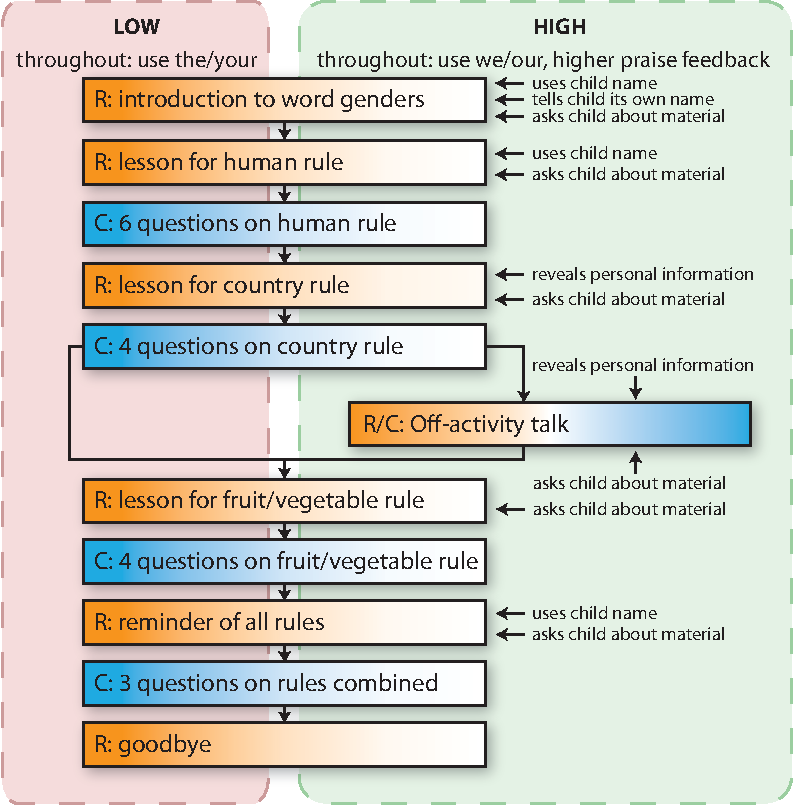
\includegraphics[width=0.75\textwidth]{images/ch9_TaskStructure_v2.pdf}
    \caption{Structure of the task. \textit{R} refers to robot explanation sections and \textit{C} refers to child question answering sections. The robot dictates the structure of the interaction through speech and by presenting questions on the touchscreen, informing the child of when it is their turn answer questions on the screen. The HIGH condition includes many manipulations in the verbal behaviour to make it more `available'.}
    \label{fig:taskstruct}
\end{figure}

All feedback was provided verbally by the robot; no feedback was shown on the screen. When providing feedback, the robot's TTS would switch to French so that the child could hear the correct pronunciation. The robot was autonomous throughout, except for some short vocal phrases in one condition, which were triggered by the experimenter (see Section \ref{sec:verbal-conds}).

%%%%%%%%%%%%%%%%%%%%%%%%%%%%%%%%%%%%%%%%%%%%%%%
\section{Evaluation} \label{sec:verbal-eval}
\subsection{Participants}\label{sec:verbal-participants}
A total of 67 children were included in the study after exclusions due to technical issues (1 child) or absence from school during one of the two visiting periods (7 children). All children were native English speakers and were from the same year group (with three class teachers) from a primary school in the U.K. (average age \textit{M}=8.8, \textit{SD}=0.4; 30M, 37F). Only one child was fluent in another language (this language was not used in this study). Children were distributed randomly between groups whilst balancing for gender and class teacher. All children had parental/guardian permission and gave their consent to take part in the study.

\subsection{Measures}\label{sec:verbal-measures}
Learning was measured through pre-, post- and retention tests, which can be seen in Appendix \ref{app:frenchtest}. These tests sought to examine various aspects of the children's learning, including their vocabulary acquisition, and their ability to apply each of the 3 rules in isolation and combination with each other. The test consisted of 12 questions: 3 vocabulary-based (1 French-English and 2 English-French), 2 about humans (rule 1), 2 about countries (rule 2), 3 about fruits and vegetables (rule 3), and 2 combined all three rules. Each question had 4 multiple choice answers and used the same formats as questions on the touchscreen. The majority of the test questions used words that the children had not seen in the learning material in order to ensure generalised \gls{learning} was taking place, rather than memorisation of specific instances; exceptions are discussed in Section \ref{sec:verbal-discussion}. The pre-, post- and retention-tests were all the same as this was necessary to account for children's prior knowledge (they had learnt some French vocabulary in school before), and to accurately measure their recall. The children were not given any feedback on their tests at any stage.

The child's perception of the robot was measured through a questionnaire combining \gls{verbalimm} and \gls{nonverbalimm} items. This 23 question questionnaire was completed on paper and was multiple choice. The \gls{verbalimm} and \gls{nonverbalimm} items were based on those used in \citet{wilson2007immediacy}, but were modified such that the language could be understood by children. The final questionnaire used can be seen in Appendix \ref{app:riq}. Verbal immediacy includes aspects of behaviour such as personalisation, off-activity talk, and student opinion solicitation. Nonverbal immediacy covers overt social behaviours, such as whether gestures are used, whether the robot looks at the child, and so on.

\subsection{Conditions and Robot Behaviour}\label{sec:verbal-conds}
In order to address the hypothesis in Section~\ref{sec:verbal-hyp}, three conditions were devised: 1) a robot with high \gls{verbalimm} (HIGH, \textit{n}=20), 2) a robot with low \gls{verbalimm} (LOW, \textit{n}=20), 3) a control with no robot and just a pre- and retention test (CTRL, \textit{n}=27). The robot with low \gls{verbalimm} doesn't have the verbal behaviours which lead to being considered available as defined by \gls{verbalimm} (Figure \ref{fig:taskstruct}). The control condition is used to verify that there are no \gls{learning} effects due to exposure to the test material.

In both robot conditions, the nonverbal behaviour was kept constant. The behaviour used was designed to be of high \gls{nonverbalimm}, with the robot's gaze randomly moving in the direction of the child, gestures during speech, a slight lean forward of the body, and slight motor noise in the arms to give the impression of being relaxed. The perception of this behaviour as being of high \gls{nonverbalimm} is verified through the questionnaire after the interaction (as described in Section \ref{sec:verbal-measures}).

The speech of the robot was kept the same in both conditions outside of the experimental manipulations as described below. This ensures that the lesson content is largely unchanged between conditions, although the experimental manipulations require some language adjustments, these should not impact on the coherence or intelligibility of the lessons.

The \gls{verbalimm} questionnaire \citep{gorham1988relationship} introduced in Chapter \ref{chap:method} was used to create the robot conditions with different immediacy levels. In order to generate the behaviour for the conditions, all of the \gls{verbalimm} questionnaire items possible were applied to the speech for the HIGH condition, and were not applied for the LOW condition. The following differences were present in the HIGH condition robot behaviour, but not in the LOW condition:
\begin{enumerate}
\item use the child's name (3 times)
\item tell the child its name
\item reveal personal information about itself (twice in addition to its name)
\item ask the child how they felt about the material (e.g., ``does everything make sense to you so far?'' 6 times)
\item ask the child about their hobbies and continue the discussion for 2 or 3 speech turns
\item use ``we/our'' work (as opposed to ``the/your'', throughout)
\item provide higher praise feedback (e.g., ``You're doing really well! That was right'', as opposed to simply ``That was right'' in the LOW condition)
\end{enumerate}

Two items of the \gls{verbalimm} questionnaire were not manipulated: humour and feedback provision. Humour was considered to be inappropriate to add given the context of the interaction and difficulties in selecting a comment that would be universally funny. Whether or not feedback was provided was not manipulated between conditions as in this context, the only way of getting feedback was from the robot and missing feedback here would confound any findings related to \gls{learning}.

To compensate for unreliable speech recognition, a Wizard-of-Oz intervention was used in the HIGH condition to let the robot reply `that's great' after the children answered a question from the robot about their understanding of the material (children always said they had understood the lesson), and to trigger pre-scripted phrases at the appropriate time for the discussion about the child's hobby. A video figure demonstrating the differences between the conditions can be seen online via the ACM digital library: \url{http://dl.acm.org/citation.cfm?id=2906873}; follow links to 'Source Materials' and then 'suppl.mov'.

\subsection{Procedure}\label{sec:verbal-proc}
The interactions took place in a quiet working space on the school premises familiar to the children. The child sat across from an Aldebaran NAO with a 27 inch touchscreen placed horizontally between them (Figure \ref{fig:snapshot}). Two video cameras were used to record the interactions. One experimenter sat behind and to the side of the child, out of their view (Figure \ref{fig:schematic}). The time children spent interacting with the robot was on average \textit{M}=11min 26s (\textit{SD}=1min 11s).

\begin{figure}[t!]
    \centering
    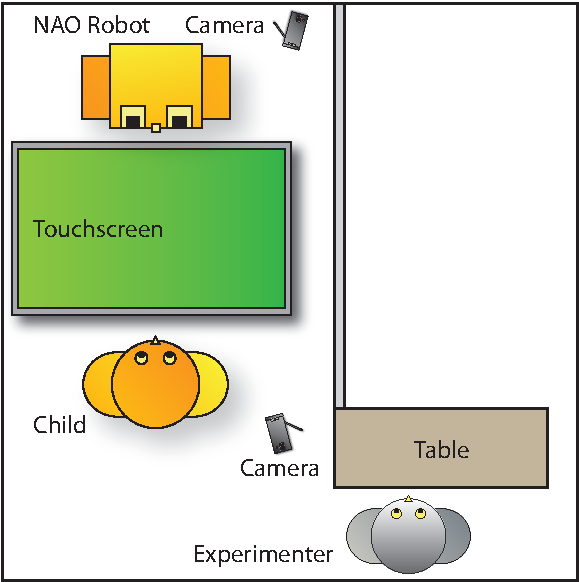
\includegraphics[width=0.5\textwidth]{images/ch9_Schematic.pdf}
    \caption{Schematic overview of the interactions being investigated in this paper. The child and the Aldebaran NAO robot sit across a touchscreen from one another. An experimenter sits behind and out of view of the child. Two video cameras record the interaction. Figure not to scale.}
    \label{fig:schematic}
\end{figure}

The experimenter spent a full week in the school, plus one day the following week. On the first Monday of the visit, pre-tests were delivered to all children in their main classrooms. These were completed under the supervision of the experimenter and the class teacher to make sure that children completed them individually. Throughout the week those children interacting with the robot would be taken out of class individually, take part in the interaction, and then complete the post-interaction test and questionnaire on paper, to the side of where the experimenter had been sitting (so they can no longer see the robot or touchscreen). The robot condition was switched between each interaction to ensure a balance throughout the week.

On the Monday of the following week the experimenter returned to deliver the retention test to the children under the same conditions as the pre-test. Children in the control group therefore completed a pre-test and a retention test without any teaching input. The children had not been informed that they would be tested again on the material that they had covered with the robot. After each class had completed the retention test, the experimenter gave an overview of the study and a presentation of social robots to all children. This meant that all children understood the study and had the opportunity to interact with the robot.

%%%%%%%%%%%%%%%%%%%%%%%%%%%%%%%%%%%%%%%%%%%%%%%%%%%%%%%%%%%%%%%%%%%%%%%%%%%%%%
\section{Results} \label{sec:verbal-results}
\subsection{Perception of the Robot}\label{sec:verbal-res-perc}
To verify that children perceive differences in the \gls{verbalimm} of the robot, the results of the post-interaction questionnaire were analysed. The questionnaire is broken down into the several parts which measure different constructs, as described in Section~\ref{sec:verbal-measures}. The manipulations were conducted on the \gls{verbalimm} element of the questionnaire. An unpaired \textit{t}-test is used to compare between the two independent robot condition groups (Kolmogorov-Smirnov test reveals no significant deviation from normality, $\textit{p}>.05$; Levene's test indicates homogeneity of variances, $\textit{p}>.05$). The test reveals a significant difference between the average \gls{verbalimm} measure for the LOW condition (\textit{M}=31.2, 95\% CI [28.1,34.3]) and the HIGH condition (\textit{M}=44.9, 95\% CI [41.6,48.2]); \textit{t}(38)=6.322, \textit{p}$<$.001. This confirms that the children could indeed perceive the difference between the conditions (despite not having seen the other condition for comparison).

Nonverbal immediacy scores were also compared using the same statistical test; the difference between the \gls{nonverbalimm} score in the LOW condition (\textit{M}=18.5, 95\% CI [17.0,19.9]) was not found to be significantly different to that of the HIGH condition (\textit{M}=19.6, 95\% CI [17.8,21.3]); \textit{t}(38)=1.020, \textit{p}=.314 (Figure \ref{fig:immgraph}). This provides some validation for the control of nonverbal behaviour between the conditions.

\begin{figure}[t!]
    \centering
    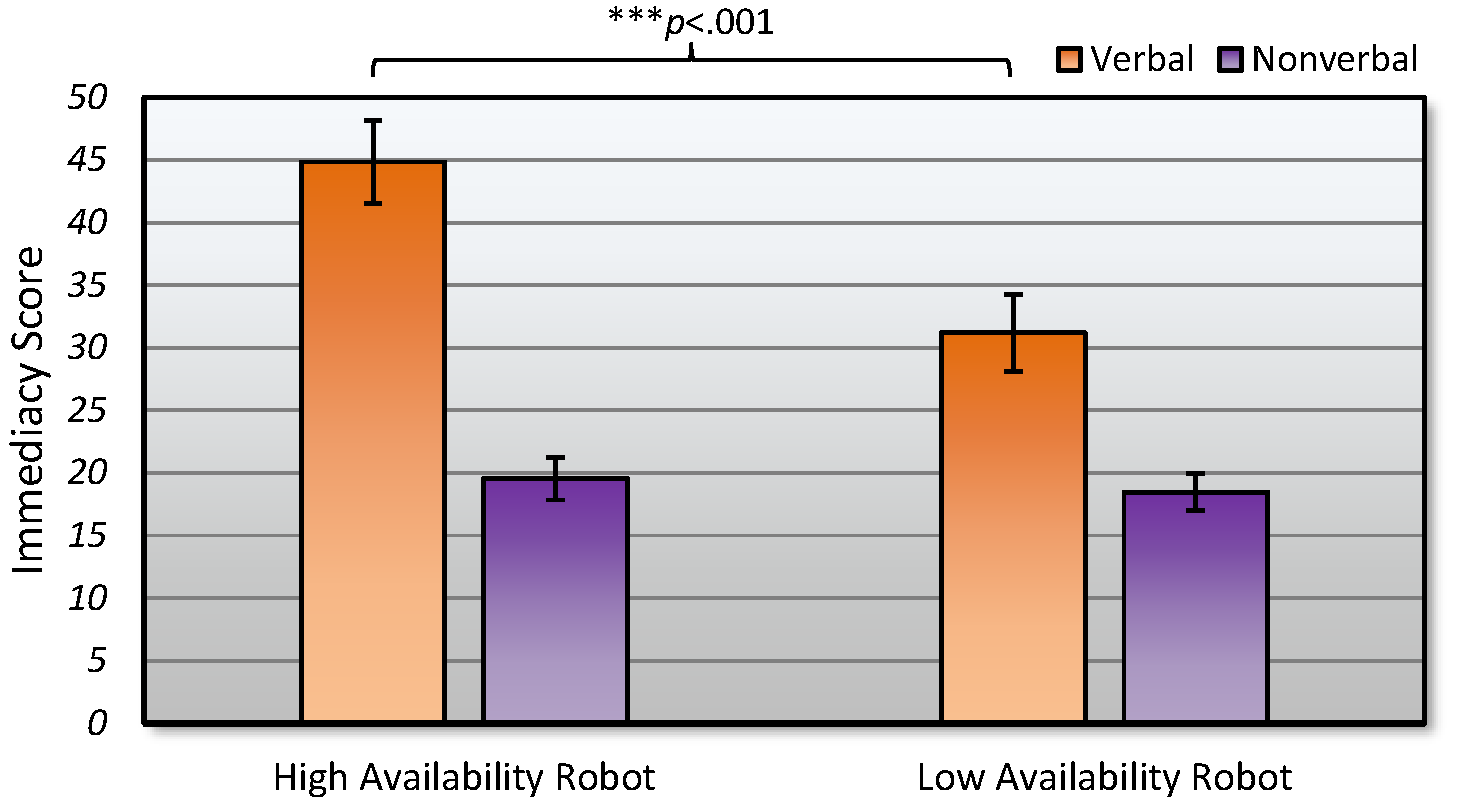
\includegraphics[width=0.7\textwidth]{images/ch9_ImmediacyGraph.pdf}
    \caption{Verbal and nonverbal immediacy scores for the high immediacy (HIGH) and low immediacy robot (LOW) conditions. The HIGH condition is perceived to have significantly higher \gls{verbalimm} while having the same \gls{nonverbalimm}. \textit{Error bars} show 95\% CI.} 
    \label{fig:immgraph}
\end{figure}

\subsection{Learning Gains}\label{sec:verbal-res-learn}
Learning gains are measured through scores on the tests conducted before the interaction (pre-test), immediately after the interaction (post-test), and 3-7 days after the interaction (retention test). Questions on the tests are equally weighted, so scores are out of a maximum of 12. Before analysis of the two robot conditions can be conducted there are some potential confounds which must be eliminated as factors: the differences in time between the interaction and retention test, and the impact of exposure to the test (as the same test is used).

It could be expected that children who interacted with the robot at a time closer to the retention test would outperform those who interacted with the robot earlier in the visit. To explore whether this was a factor, the day on which the interaction took place was correlated with the difference between the post-test and the retention test. The correlation is weak and non-significant; \textit{r}(36)=-.079, \textit{p}=.637, indicating that the time from interaction to retention test can be eliminated as a factor. It is suggested that the absolute number of days does not make a difference to the retention, but the number of days out of school during this period is more important, which was constant for all children (a weekend of 2 days).

The control condition is used to verify whether exposure to the test makes a difference to the findings. It would not be expected that there would be a difference as the children are given no feedback on the tests at any stage, but the control condition allows verification. Equivalency testing is used to demonstrate not only that there is no significant difference, but that there is significant equivalency. For children in the control condition, the pre-test score (\textit{M}=3.96, 95\% CI [3.26,4.66]) and retention test score (\textit{M}=3.89, 95\% CI [3.28,4.49]) can be considered equivalent. Two one-sided \textit{t}-tests (TOST; \citealp{schuirmann1987comparison}) with a 1 point threshold confirm the test scores are equivalent at the \textit{p}$<$.05 level: \textit{t}(52)=$-$2.061, \textit{p}=.022/\textit{t}(52)=2.391, \textit{p}=.010. This indicates that exposure to the test is not a confounding factor.

A repeated measures ANOVA was used to explore H1, that the robot condition affects \gls{learning}, in both the short-term and after a delayed period. The repeated measures ANOVA was used as each test is a matched measure for that participant; 2 levels are used so that the effect of test and condition can be explored across the continuous measure of test score. Figure~\ref{fig:testgraph} and Table~\ref{tab:results} show the results for test scores by condition. Mauchly's Test of Sphericity indicated that the assumption of sphericity had not been violated\footnote{Sphericity is an important assumption for using a repeated-measures ANOVA. Sphericity indicates equal variances of the differences between all possible pairs of groups (levels of the independent variable). If this is not the case, then variance calculations may not be accurate, producing an inflated F-ratio. Further details about Mauchly's test in particular can be seen in \citet{mauchly1940significance}.}, $\chi^2$(2)=1.873, \textit{p}=.392. No significant interaction was found between test and condition; Wilk's Lambda=.998, \textit{F}(2,35)=0.04, \textit{p}=.963. A main effect was found for test, Wilk's Lambda=.391, \textit{F}(2,35)=27.21, \textit{p}$<$.001, but not for condition; \textit{F}(1,36)=0.08, \textit{p}=.774. Bonferroni pairwise comparisons find that there is a significant difference between pre-test and post-test, and pre-test and retention test scores (all \textit{p}$<$.001), but no difference between post-test and retention test (\textit{p}=1.00).

These results do not support H1, as children learn between the pre- and post-tests, and retain their \gls{learning} in the retention test, but this does not differ by robot condition. Further to this, Weber \& Popova paired-samples equivalency tests \citep{weber2012testing}\footnote{The Weber \& Popova equivalency tests consider paired samples, whereas the TOST equivalency technique previously used is appropriate for independent samples.} show that the post and retention test scores are equivalent in both the HIGH (\textit{t}(18)=0.67, \textit{p}=.022) and LOW (\textit{t}(18)=0.73, \textit{p}=.025) conditions, with Cohen's \textit{d}=.50. Whilst this is an `intermediate' effect size for demonstrating equivalency, it should be noted that the sample size is relatively small on a per-condition basis, leading to a higher variation in scores, which raises the level at which equivalency can be shown. Combined, these findings suggest that the children learn a significant amount from the pre-test to the post-test, and the post-test and retention test scores can be considered largely equivalent, demonstrating their retention of the \gls{learning} in both conditions.

The ANOVA results do not support H1 (that higher immediacy will lead to greater \gls{learning}) as no significant effect was found for robot condition. Nor can a significant difference be seen between the improvement in the LOW condition (\textit{M}=3.80, 95\% CI [2.55,5.05]) and the HIGH condition (\textit{M}=3.35, 95\% CI [1.78,4.92]); \textit{t}(38)=0.470, \textit{p}=.641. The drop in score from post-test to retention test can also be considered equivalent between conditions; using a Weber \& Popova independent-samples equivalance test, \textit{t}(36)=0.07, \textit{p}=.004 with Cohen's \textit{d}=.50. Therefore, Hypothesis H1 must be rejected as there are no significant differences observed between conditions in terms of \gls{learning}.

\begin{figure}[t!]
    \centering
    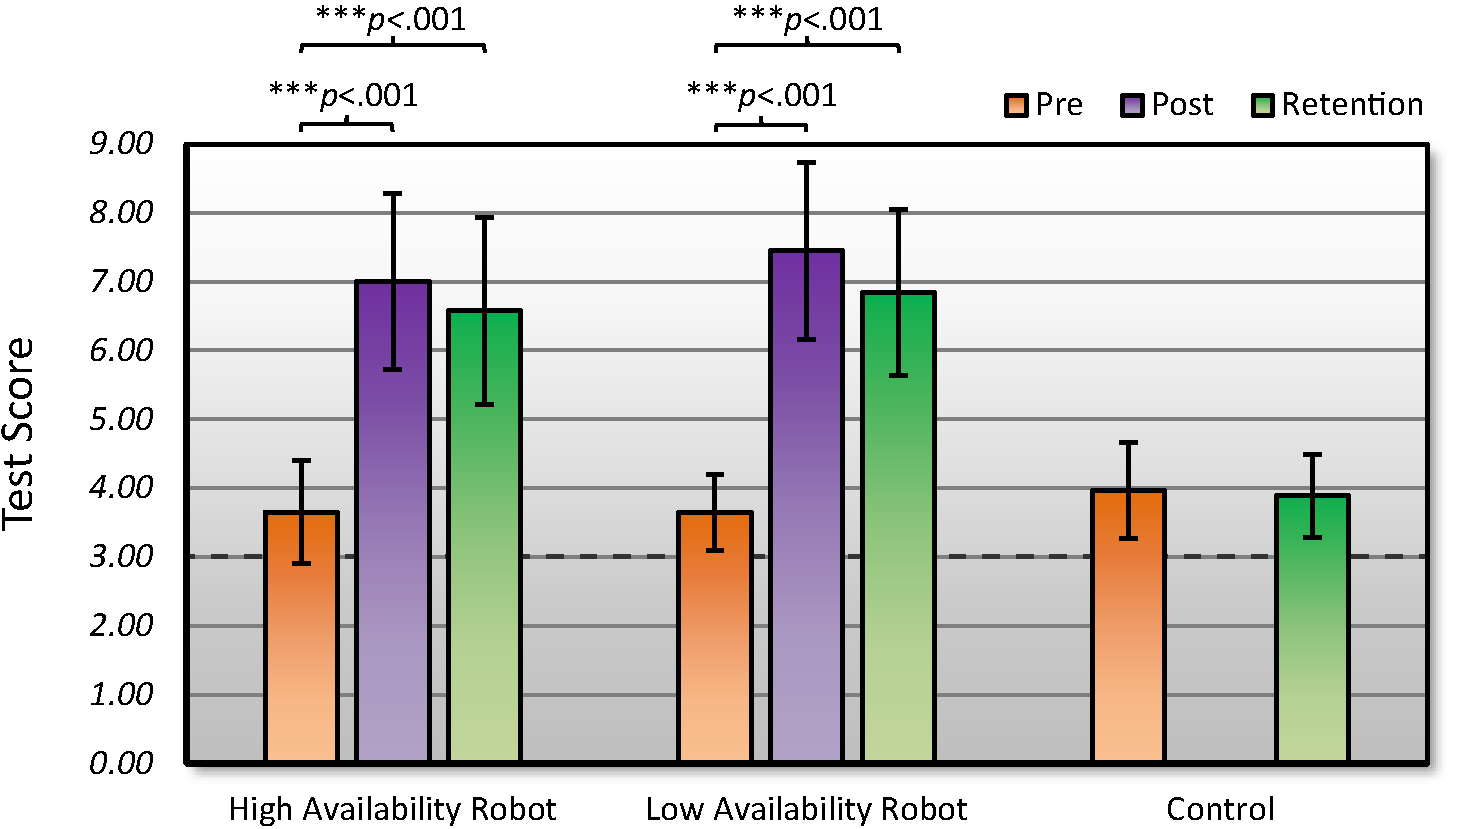
\includegraphics[width=0.9\textwidth]{images/ch9_TestGraph.pdf}
    \caption{Pre-test, post-test and retention test scores by condition (chance score=3; maximum score=12). Children learn a significant amount from the robot between pre- and post-tests; this gain is sustained to the retention test. \textit{Error bars} show 95\% CI. Darker dashed line indicates the `chance' baseline.}
    \label{fig:testgraph}
\end{figure}

\begin{table}[t!]
\centering
\renewcommand{\arraystretch}{1.2} 
\begin{tabular}{@{}llll@{}}
\toprule
\textbf{Condition} & \begin{tabular}[c]{@{}l@{}}\textbf{Pre-Test} \\ \textbf{\textit{M} {[}95\% CI{]}}\end{tabular} & \begin{tabular}[c]{@{}l@{}}\textbf{Post-Test} \\ \textbf{\textit{M} {[}95\% CI{]}}\end{tabular} & \begin{tabular}[c]{@{}l@{}}\textbf{Retention Test} \\ \textbf{\textit{M} {[}95\% CI{]}}\end{tabular} \\ \midrule
CTRL      & 3.96 {[}3.26, 4.66{]}                                               & N/A                                                                  & 3.89 {[}3.28, 4.49{]}                                                     \\
LOW       & 3.65 {[}3.10, 4.20{]}                                               & 7.45 {[}6.17, 8.73{]}                                                & 6.84 {[}5.64, 8.05{]}                                                     \\
HIGH      & 3.65 {[}2.90, 4.40{]}                                               & 7.00 {[}5.72, 8.28{]}                                                & 6.58 {[}5.22, 7.94{]}                                                     \\ \bottomrule
\end{tabular}
\caption{Test score results for pre-test, post-test and retention tests, by condition.}
\label{tab:results}
\end{table}

Based on the rules taught to the children, one could suggest that learning a very simple rule of: ``if the word ends in an `e', then use \textit{la}, otherwise use \textit{le}'' may be adopted as a `shortcut' and could account for the \gls{learning} differences. This would then have nothing to do with learning aspects of language, but be a basic memory phenomenon. This had been anticipated in the study design, so later questions in the learning material made sure to challenge this approach by including several words ending in `e' as possible answers, but with those words relating to humans of male gender (therefore requiring `le', rather than `la' and violating the shortcut rule). Additionally, a question in the tests used adopted this approach, with several words ending in an `e', but not all being feminine. This was done to verify whether the shortcut rule had been adopted, or whether the children had really learnt the material as it had been taught, with the ability to discriminate between different types of words. If the children had only learnt the shortcut rule then they would answer this verification question incorrectly, however, it was answered correctly above the average level for the rest of the questions in the test (63\% for the verification question, versus 60\% for the other questions). This provides some evidence that the children learnt intricacies of the language that was presented to them; further evidence in support of this will be provided in Section \ref{sec:verbal-discussion}.

%%%%%%%%%%%%%%%%%%%%%%%%%%%%%%%%%%%%%%%%%%%%%%%%%%%%%%%%%%%%%%%%%%%%%%%%%%%%%%
\section{Discussion} \label{sec:verbal-discussion}
The results show that the children perceived the \gls{verbalimm} of the robot conditions as intended, which confirms that the behaviour was designed appropriately to address the research hypothesis. The nonverbal behaviour was kept constant between the two conditions, and this was reflected in the children's questionnaire responses. The children in both robot conditions exhibited significant \gls{learning} gains between the pre-test and post-test, as well as between the pre-test and retention test, with equivalent scores in the retention test and the post-test. This is a positive result, as it would have been plausible that the children would quickly forget what the robot had taught them once the interaction was over, especially as the children were not aware that they would be re-tested, and so had little motivation to attempt to actively try and retain the information.

The tests which the children had to complete were designed to be challenging. Each answer had four options with no obviously incorrect answers, so the likelihood of a guess being correct would be chance (25\%). It was found that children scored slightly above this on the pre-tests as they had done a small amount of French before, so scored closer to 4 than the 3 that would be expected with random guessing. This significantly improved to over 7 out of 12 in the post-tests. Given the difficulty of the tests and the relatively short time the child interacts with the robot learning and practising the material, this is an impressive increase. Indeed, only 6 of the 40 children who interacted with the robot did not improve from pre-test to post-test. Learning of `le' or `la' as the article choice could have contributed to part of the increase in scores, however if children had learnt the choice to be le/la then the chance score would go up by 1.5 points from pre-test (chance = 3) to post-test (chance = 4.5). The children actually improve by an average of 3.6 (95\% CI [2.6,4.5]), suggesting \gls{learning} beyond any improvement due to the higher chance score.

Despite the children being able to perceive the difference in verbal aspects of immediacy between the two robot conditions (measured through \gls{verbalimm}), no significant difference was observed in \gls{learning} in either the post- or retention-test. This finding is surprising given the positive correlation between \gls{verbalimm} and \gls{learning} in human studies \citep{gorham1988relationship,witt2004meta}. The high \gls{verbalimm} robot condition was perceived to have significantly higher \gls{verbalimm}, but this did not translate into additional \gls{learning} gains as expected. The content of the lessons was the same, but the difference to \gls{learning} that social behaviour can make has previously been demonstrated in HRI in spite of the same content between conditions for nonverbal behaviour \citep{kennedy2015higher,szafir2012pay}. However, the learning material here is different to prior work, so it is possible that the content under consideration interacts with the robot social behaviour, influencing the \gls{learning} effects.

Aspects of the behaviour manipulated here, such as personalisation \citep{henkemans2013using} and off-activity talk \citep{kruijff2014oat}, have been studied before in HRI with promising results. However, these studies had too few subjects to make conclusions about learning \citep{henkemans2013using}, or did not assess learning \citep{kruijff2014oat}. In contrast to \cite{kruijff2014oat}, the children here do perceive differences between the conditions, but in this study the questionnaire is targeted towards specifically measuring the perception of the behaviours which were manipulated, rather than assessing an overall feeling towards the robot. It is possible that despite children perceiving differences in the immediacy of the robot, this did not translate into any difference in feeling towards the robot. If the relationship the child feels towards the robot is no different between conditions then this may go some way to explaining the lack of difference in \gls{learning}.

The interpretation of the robot character could have been influenced by the TTS voice used by the robot, which would switch when the language changed. These voices were clearly different and this could have impacted how the children perceived the robot. However, the children have no prior experience with the robot, so they may have accepted this as part of the robot's behaviour. As the voices are clearly different, they may also have interpreted this not to be part of the robot's character, but to be the robot playing back other media (akin to a teacher playing recorded French). It is not possible to determine how the children perceived this switch in voice from the data collected, but perceptions of voice switching of multi-lingual robots could be worth explicitly exploring in future work.

Another factor which may have influenced the \gls{learning} results is novelty. Novelty is often an issue for HRI studies \citep{leite2013social,sung2009robots}, and it possibly played a role here as the children interact just once with the robot for a brief period of time. Verbal immediacy has been found to consist of four factors, including `individual friendliness' \citep{wilson2007immediacy}. Even if the children were to bond more strongly with the high immediacy robot because of increased friendliness, the short interaction time might not be enough for differences in the relationship to manifest into \gls{learning} outcomes. Furthermore, it could be that the behaviour of the more available robot cancels out its own benefits by being so novel as to distract from the learning material. For example, when the robot is conducting off-activity talk during the interaction, this is time when the children are not focussing on the learning task and are possibly forgetting information they have learnt. This doesn't mean that off-activity talk should be avoided for fear of distraction, but that it might only be appropriate in longer, or repeated interactions where novelty is less of an issue. It is hypothesised that given a longer interaction timescale, the \gls{learning} benefits predicted by the literature of greater immediacy \citep{gorham1988relationship,witt2004meta} would be observed as the novelty wears off \citep{kanda2004interactive,leite2013social}.

In the HHI literature, a lower correlation between \gls{verbalimm} and \gls{learning} has been found when compared to \gls{nonverbalimm} and learning \citep{witt2004meta}. Nonverbal immediacy has previously been found to make a difference to learning in HRI \citep{kennedy2015higher,szafir2012pay}. This could suggest that verbal behaviour may not be as important for \gls{learning} (at least in short-term interactions) as overt nonverbal behaviour. It has also been found in humans that the impact of immediacy behaviours is enhanced in line with increases in class size \citep{gorham1988relationship}. It could be that the effect of \gls{verbalimm} is simply too far reduced when placed in a one-to-one tutoring context as in this study, rather than the larger classroom setting. The immediacy of the robot would be experienced to some extent in both conditions simply through the nature of the one-to-one interaction.

One interesting finding from the data collected which was not hypothesised was the ability of the children to acquire vocabulary despite the learning material not explicitly requiring them to do so. Three questions of the test were vocabulary based: two requiring translation from English to French, and one French to English. Two of these questions referred to words which the children would have seen on screen and heard the robot say (as they were answers to questions in the learning material). The remaining question was about a word which they would have seen on screen, but the robot did not say (as it was not a correct answer). It is suggested that the two words which were answers in the learning material were more likely to be recalled as the children would have looked at the word for longer and the robot would have said the word. However, a significant increase was found for all 3 of the questions independently, and a repeated measures ANOVA found a significant increase for the average score (out of 3) of children who correctly translated the words from pre-test to post-test, and from pre-test to retention test. Mauchly's Test of Sphericity indicated that the assumption of sphericity had not been violated, $\chi^2$(2)=0.661, \textit{p}=.719. No significant interaction was found between test and condition; Wilk's Lambda=.968, \textit{F}(2,35)=0.58, \textit{p}=.565. A main effect was found for test, Wilk's Lambda=.595, \textit{F}(2,35)=11.94, \textit{p}$<$.001, but not for condition; \textit{F}(1,36)=0.14, \textit{p}=.710. Post-hoc Bonferroni pairwise comparisons find that there is a significant difference between pre-test (\textit{M}=0.8, 95\% CI [0.6,1.0]) and post-test (\textit{M}=1.6, 95\% CI [1.3,1.9]), and pre-test and retention test (\textit{M}=1.4, 95\% CI [1.1,1.7]) scores (\textit{p}$<$.001 and \textit{p}=.001, respectively), but no difference between post-test and retention test scores (\textit{p}=.883).

It is of course possible that the children remembered the words from the pre-test and made an effort to learn these words when they were presented on screen, but this seems unlikely given the time (up to 4 days) between many of the pre-tests and the interactions, and the sheer number of words they were exposed to in the learning content (over 40). For a child to concentrate on learning 3 words from the pre-test, days after having seen it, when being taught a different aspect of language would seem to be highly improbable. As such, this is a promising finding with robots that confirms data from human-human literature whereby children of this age will acquire language through exposure in social interactions \citep{kuhl2010brain}.

%%%%%%%%%%%%%%%%%%%%%%%%%%%%%%%%%%%%%%%%%%%%%%%%%%%%%%%%%%%%%%%%%%%%%%%%%%%%%%
\section{Summary} \label{sec:verbal-summary}
Children perceived the relative \gls{verbalimm} of the two robot conditions as intended in the design. This confirms that the manipulations made were appropriate to address the question of whether an increase in verbal aspects of immediacy would lead to an increase in \gls{learning}. As expected, the children did learn elements of a second language from the robot. This was measured immediately after the interaction and also some days later. The retention test scores were slightly lower than the pre-test scores, but can be considered statistically equivalent. However, surprisingly there was a lack of any significant difference between conditions in the immediate post-test score, or the longer-term retention test score. Literature from human-human interaction studies \citep{gorham1988relationship,witt2004meta} and human-robot interaction studies \citep{henkemans2013using,kruijff2014oat} would predict an increase in robot \gls{verbalimm} to lead to an increase in \gls{learning}, but this was not found. It is suggested that in this short-term dyadic interaction context, additional effort in developing social aspects of a robot's verbal behaviour may not return the desired positive impact on \gls{learning} gains.